\chapter{Phương pháp đề xuất}
\label{Chapter3}

\section{Cơ sở lý thuyết}
Phần này trình bày chi tiết về cơ sở lý thuyết, các khái niệm cần thiết liên quan đến đề tài nghiên cứu.
\subsection{Kiến trức IoT bốn lớp}
\label{sec:4layer}
Một kiến trúc IoT điển hình bao gồm bốn thành phần chính: phần phần cứng được kết nối (các “thiết bị thông minh”) có nhiệm vụ thu thập và xử lý dữ liệu thông qua cảm biến hoặc bộ điều khiển tại thiết bị biên, kết nối truyền thông (có thể gồm nhiều giao thức), đảm bảo việc truyền nhận dữ liệu giữa thiết bị và nền tảng đám mây; hệ thống xử lý dữ liệu – thường tích hợp trong nền tảng điện toán đám mây; và cuối cùng là ứng dụng trực quan hóa dữ liệu thu thập được.
\begin{figure}[h]
    \centering
    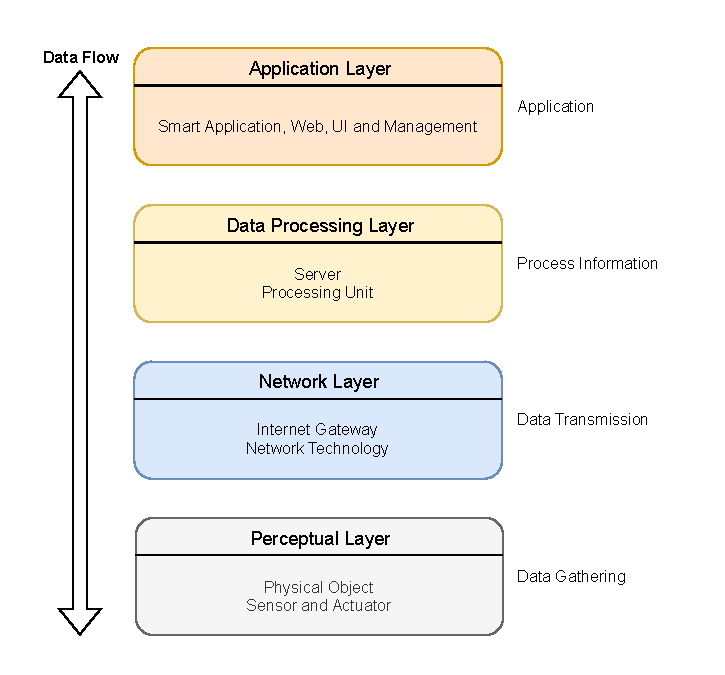
\includegraphics[width=0.75\linewidth]{images/4layer.pdf}
    \caption{Mô hình IoT 4 lớp}
    \label{fig:4layer}
\end{figure}
\subsubsection{Lớp nhận thức (Perceptual Layer)}
Đây là lớp đầu tiên của hệ thống, có nhiệm vụ thu thập dữ liệu từ nhiều nguồn khác nhau. Lớp này bao gồm các cảm biến được đặt trong môi trường nhằm thu thập dữ liệu về nhiệt độ, độ ẩm, ánh sáng và các dữ liệu vật lý khác. Các chuẩn giao tiếp có dây hoặc không dây thường được sử dụng để kết nối với lớp gateway ở trên.
\subsubsection{Lớp mạng (Network Layer)}
Lớp mạng thường được sử dụng như một gateway nhằm đảm bảo kết nối và truyền thông giữa các thiết bị IoT cũng như với mạng internet. Các công nghệ như Wi-Fi, Bluetooth, Zigbee, hoặc mạng di động (4G, 5G) được sử dụng, cùng với các cổng (gateway) như ESP32 sẽ được dùng để chuyển tiếp dữ liệu. Lớp này thường sử dụng các cơ chế mã hóa dữ liệu để đảm bảo an toàn trong quá trình truyền dữ liệu.
\subsubsection{Lớp xử lý dữ liệu (Data Processing Layer)}
Lớp xử lý dữ liệu thường là các máy chủ (server) trung gian có vai trò thu nhận, phân tích, và xử lý dữ liệu thô từ các thiết bị IoT. Các công cụ như hệ quản trị dữ liệu, nền tảng phân tích, hoặc thuật toán học máy được sử dụng để trích xuất thông tin giá trị. Lớp này cũng có vai trò xác định dữ liệu nhận từ các thiết bị có chính xác hay không, từ đó quyết định xem nên lưu trữ dữ liệu hay từ chối nhận dữ liệu từ bên ngoài.
\subsubsection{Lớp ứng dụng (Application Layer)}
Đây là lớp cao nhất, cung cấp giao diện thân thiện cho người dùng để tương tác với hệ thống IoT. Bao gồm các ứng dụng di động, web, và phần mềm trung gian (middleware) cho phép tích hợp và chia sẻ dữ liệu giữa các thiết bị.

\subsection{Giao thức MQTT}
Trong hệ thống IoT được xây dựng, giao thức được sử dụng để giao tiếp giữa gateway và máy chủ là giao thức MQTT (Message Queuing Telemetry Transport). Đây là một giao thức nhắn tin nhẹ, tối ưu cho các ứng dụng IoT, nơi yêu cầu truyền dữ liệu nhanh, gọn và tiêu tốn ít tài nguyên. Trong kiến trúc MQTT, Broker đóng vai trò là trung tâm phân phối thông điệp giữa các thiết bị, giúp chúng gửi và nhận thông điệp thông qua mô hình publish/subscribe. Khi một thiết bị publish một thông điệp đến một chủ đề (topic), Broker sẽ tiếp nhận và chuyển thông điệp đó đến mọi thiết bị đã subscribe topic tương ứng. Ngoài việc chuyển tiếp dữ liệu, Broker còn chịu trách nhiệm quản lý kết nối của các thiết bị, xử lý cơ chế giữ kết nối, và duy trì trạng thái phiên làm việc của client. 

\begin{figure}[h]
    \centering
    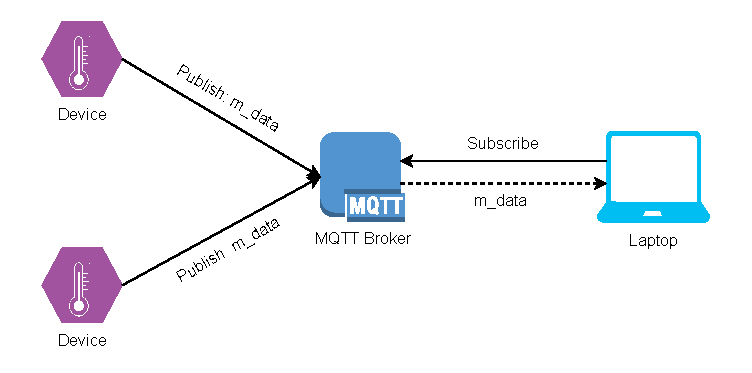
\includegraphics[width=0.85\linewidth]{mqtt.pdf}
    \caption{Giao thức MQTT}
    \label{fig:mqtt}
\end{figure}

\subsection{Mật mã hóa nhẹ ASCON-128a}
% \subsubsection{Giới thiệu về ASCON-128a}
Trong các hệ thống IoT hạn chế tài nguyên, việc sử dụng các thuật toán mã hóa truyền thống như AES hoặc RSA thường gặp nhiều bất cập do yêu cầu cao về năng lượng và khả năng tính toán. Điều này dẫn đến độ trễ lớn và tiêu tốn tài nguyên, ảnh hưởng đến hiệu quả hoạt động của các thiết bị nhúng. Trước thực trạng đó, mã hóa nhẹ (lightweight cryptography) đã được nghiên cứu và phát triển như một giải pháp tiềm năng, nhằm cung cấp mức độ bảo mật phù hợp với chi phí tính toán thấp.

% Gần đây, nhiều công trình nghiên cứu đã tập trung vào việc thiết kế và đánh giá các thuật toán mã hóa nhẹ, trong đó có Ascon và các biến thể tối ưu của AES, nhằm đáp ứng yêu cầu bảo mật cho các ứng dụng IoT. Nổi bật trong số đó là Ascon – thuật toán đã được Viện Tiêu chuẩn và Công nghệ Hoa Kỳ (NIST) lựa chọn làm tiêu chuẩn cho mã hóa nhẹ vào năm 2023 \cite{1984-TeX-Knuth}. Ascon là một thuật toán mã hóa xác thực kèm dữ liệu liên kết (Authenticated Encryption with Associated Data – AEAD), được thiết kế để đảm bảo mức độ bảo mật cao, hiệu suất xử lý tối ưu và cấu trúc đơn giản. Nhờ vào số lượng cổng logic thấp và khả năng chống chịu mạnh mẽ trước các tấn công mật mã học, Ascon trở thành một lựa chọn lý tưởng cho các thiết bị IoT có hạn chế về tài nguyên.

Các công trình gần đây, chẳng hạn như bài báo \cite{AESvsAscon} đã triển khai hệ thống IoT ứng dụng cho y tế đã so sánh 2 thuật toán mã hóa là Ascon-128 và AES-GCM-128 trên Raspberry Pi. Kết quả cho thấy Ascon-128 cho ra hiệu suất tốt hơn hoàn toàn so với AES-GCM-128 về mặt hiệu năng. Bài báo thực hiện so sánh tốc độ mã hóa của từng gói tin với kích thước khác nhau, Ascon cho ra hiệu suất cao với các gói tin có kích thước nhỏ, chẳng hạn với 8 byte dữ liệu, Ascon có hiệu suất gấp 8 lần so với AES và với 1024 byte, Ascon có hiệu suất gấp đôi. Với 2048 byte, Ascon vẫn cho ra hiệu suất tốt hơn dù mức độ chênh lệch không nhiều, hình \ref{fig:ascon-aes} được trích ra từ bài báo thể hiện hiệu suất của Ascon-128 so với phương pháp AES.

\begin{figure}[h]
    \centering
    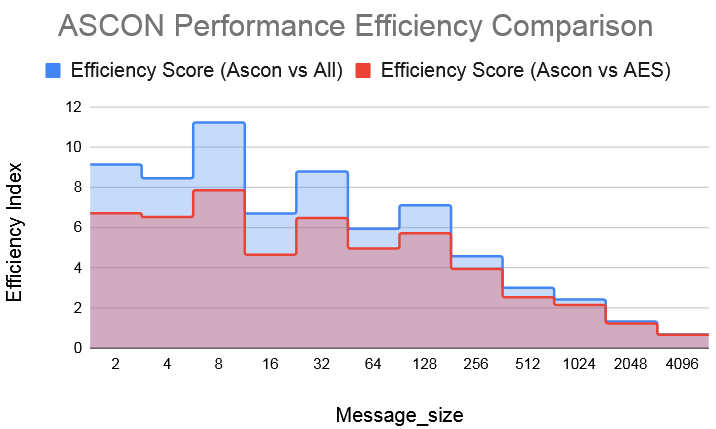
\includegraphics[width=0.7\linewidth]{ascon-aes.png}
    \caption{So sánh hiệu năng giữa Ascon và AES được trích từ bài báo}
    \label{fig:ascon-aes}
\end{figure}

Một nghiên cứu khác từ Dobraunig et al. (2021) trong bài giới thiệu Ascon v1.2 cũng nhấn mạnh hiệu suất cao của Ascon-128 khi thực hiện mã hóa dữ liệu có kích thước vừa và nhỏ so sánh với các thiết kế AES dùng native AES instruction trên Intel Skylake processors. 

NIST cũng đã thực hiện đánh giá một số thuật toán mã hóa nhẹ ở vòng chung kết. Kết quả cho thấy Ascon là thuật toán có hiệu suất tốt nhất so với các thuật toán mã hóa nhẹ khác như Elephant, Grain-128aead hoặc Sparkle. Ascon cũng đã được NIST lựa chọn làm tiêu chuẩn mã hóa nhẹ chính thức vào năm 2023 dựa vào độ an toàn cao và hiệu suất vượt trội trên cả phần mềm lẫn phần cứng trong môi trường IoT giới hạn tài nguyên. NIST thực hiện đánh giá trên các nền tảng như 8-bit AVR, ARM Cortex-M0+/M3/M4, RISC-V, Xtensa LX6, v.v. Thời gian thực thi của Ascon nhanh hơn đáng kể so với chuẩn AES-GCM trên nRF52840. Trong các thử nghiệm benchmark độc lập, Ascon là một trong số ít thuật toán đạt hiệu suất cao và footprint nhỏ nhất, đặc biệt trên thiết bị nhúng có tài nguyên hạn chế.

\subsubsection{Thuật toán ASCON-128a}
ASCON là một bộ thuật toán mã hóa nhẹ bao gồm tập hợp các thiết kế mã hóa xác thực và một họ các hàm băm cùng hàm sinh đầu ra mở rộng \cite{?}. Ở đề tài này tập trung vào phần mã hóa xác thực trong triển khai hệ thống. Vì vậy, để đảm bảo tính ngắn gọn, chỉ có mã hóa xác thực được thảo luận trong phần này. ASCON sử dụng chế độ hoạt động dựa trên cấu trúc duplex, trong đó phép hoán vị 320-bit của ASCON được lặp lại thông qua một mạng hoán vị - thay thế (Substitution-Permutation Network - SPN) để thực hiện quá trình mã hóa hoặc giải mã dữ liệu. Quá trình này được thực hiện theo kiểu bit-slice, một đặc điểm giúp ASCON có khả năng mở rộng linh hoạt trên các nền tảng xử lý 8, 16, 32 và 64 bit, đồng thời vẫn đảm bảo tính "nhẹ" của thuật toán.

ASCON có hai biến thể chính phù hợp với độ dài khối dữ liệu cần mã hóa khác nhau: ASCON-128 và ASCON-128a. Trong các thuật toán mã hóa khối (block cipher), dữ liệu đầu vào được chia thành các khối có độ dài cố định. Trong đó, ASCON-128 sử dụng khối dữ liệu 64-bit và ASCON-128a sử dụng khối dữ liệu 128-bit. Các tập tham số tương ứng của từng biến thể ASCON được trình bày trong Bảng \ref{tab:ascon_parameter}. Như thể hiện trong bảng, điểm khác biệt chính giữa các biến thể là kích thước khối dữ liệu và số vòng lặp trong quá trình hoán vị.

Quy trình mã hóa của ASCON được mô tả trong Hình \ref{fig:ascon_process}, gồm bốn giai đoạn chính:
\begin{enumerate}
    \item Khởi tạo (Initialization)
    \item Xử lý dữ liệu liên kết (Associated Data Processing)
    \item Xử lý plaintext (Plaintext Processing)
    \item Kết thúc và tạo thẻ xác thực (Finalization for Tag Generation)
\end{enumerate}

\begin{figure}
    \centering
    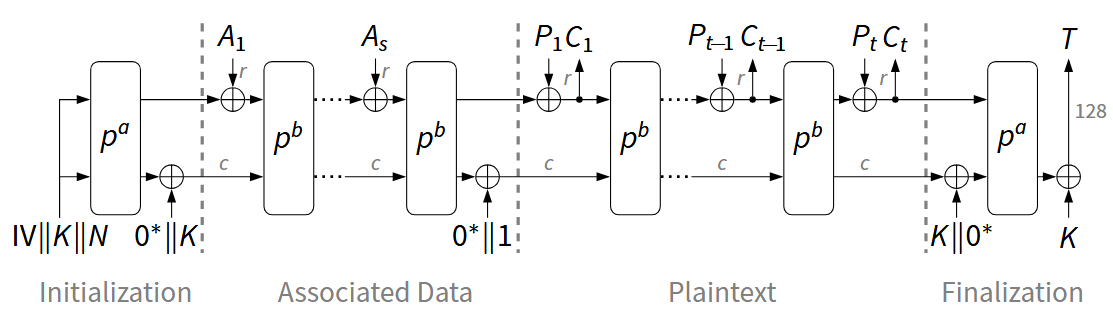
\includegraphics[width=0.9\linewidth]{ascon_process.png}
    \caption{Quá trình mã hóa của ASCON với dữ liệu liên kết}
    \label{fig:ascon_process}
\end{figure}

Trong suốt quá trình này, hai phép hoán vị 320-bit ký hiệu là $p^a$ và $p^b$ được sử dụng, trong đó $a$ và $b$ biểu thị số vòng lặp tương ứng. Các phép hoán vị này được biểu diễn theo dạng bit-slice, chia thành năm thanh ghi 64 bit, tạo thành trạng thái nội bộ gồm 5 word mỗi word có 64 bit.

Trong phiên bản ASCON đầy đủ với 12 vòng lặp, các phép hoán vị áp dụng lặp đi lặp lại quá trình biến đổi dựa trên mạng hoán vị - thay thế (SPN), bao gồm các bước: cộng hằng số vòng lặp (round constants), áp dụng lớp thay thế (substitution layer) và sử dụng lớp tuyến tính (linear layer) để khuếch tán dữ liệu trong trạng thái nội bộ.

Lớp thay thế (Substitution layer) sử dụng một hộp thế (S-box) gồm 5 bit có cấu trúc nhỏ gọn và tối ưu cho các hệ thống nhẹ, như minh họa trong Hình \ref{fig:s-box}. S-box được áp dụng song song 64 lần, nhằm cập nhật từng bit-slice trong trạng thái nội bộ. S-box 5 bit được thiết kế dựa trên login Boolean, cho phép triển khai hiệu quả trên cả hai nền tảng phần cứng ASIC và FPGA.

\begin{figure}
    \centering
    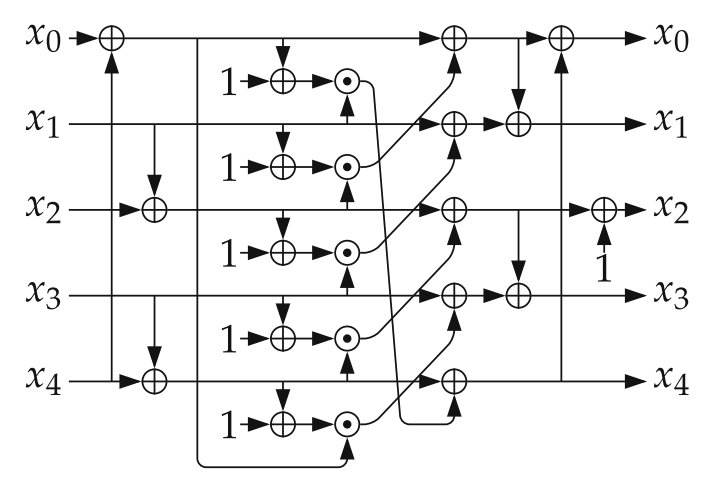
\includegraphics[width=0.6\linewidth]{s-box.png}
    \caption{Khối 5-bit S-box của ASCON}
    \label{fig:s-box}
\end{figure}

Lớp tuyến tính (Linear Layer) trong ASCON cập nhật mỗi word 64 bit trong trạng thái nội bộ bằng cách xoay (rotate) các thanh ghi với các giá trị dịch bit khác nhau, sau đó công theo modulo-2 (XOR) các giá trị đã được dịch.

Quá trình giải mã có một vài điểm khác biệt so với mã hóa. Thay vì xử lý plaintext, giải mã sử dụng hàm xử lý dữ liệu mã hóa (ciphertext processing), trong đó các khối plaintext được khôi phục bằng cách thực hiện phép XOR giữa khối plaintext và trạng thai hiện tại.

\begin{table}[ht]
\centering
\small
\caption{Bảng tham số cho ASCON}
\begin{tabular}{|p{3cm}|p{1.5cm}|p{1.5cm}|p{1.5cm}|p{2.8cm}|p{1cm}|p{1cm}|}
    \hline
    \multirow{2}{*}{Variants} & \multicolumn{4}{c|}{Bit size} & \multicolumn{2}{c|}{Rounds} \\
    \cline{2-7}
    & Key & Nonce & Tag & Data Block & $p^a$ & $p^b$ \\
    \hline
    ASCON-128 & 128 & 128 & 128 & 64 & 12 & 6 \\
    \hline
    ASCON-128a & 128 & 128 & 128 & 64 & 12 & 8 \\
    \hline
\end{tabular}
\label{tab:ascon_parameter}
\end{table}

\subsection{Thuật toán trao đổi khóa Elliptic Curve Diffie-Hellman}
\subsubsection{Đường cong Elliptic trên trường hữu hạn}
Một đường cong elliptic là một đường cong trơn (không có điểm nhọn hay tự cắt) được xác định bởi phương trình dạng
\[
    y^2 = x^3 + ax + b \pmod{p}
\]
trong đó $a$ và $b$ là các hằng số và $p$ là một số nguyên tố đại diện cho trường hữu hạn (finite field). Đường cong này có thể được diễn giải theo hình học và mang cấu trúc nhóm, cụ thể là một nhóm cộng với phép cộng điểm trên đường cong. Hình \ref{fig:curve} minh họa một đường cong elliptic với $a = -2$ và $b = 5$.

\begin{figure}[h]
    \centering
    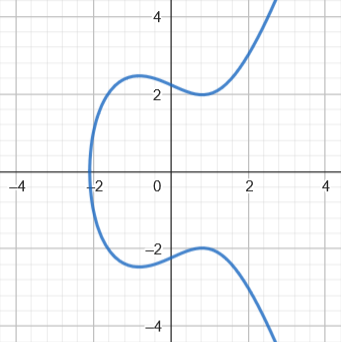
\includegraphics[width=0.4\linewidth]{curve.png}
    \caption{Đường cong elliptic $y^2 = x^3 - 2x + 5$}
    \label{fig:curve}
\end{figure}

Phép cộng hai điểm $P$ và $Q$ trên đường cong sẽ tạo ra một điểm thứ ba $R = P + Q$. Cách thực hiện là vẽ đường thẳng đi qua hai điểm $P$ và $Q$, tìm điểm giao thứ ba của đường thẳng đó với đường cong, sau đó phản xạ điểm này qua trục hoành (trục $x$) thể thu được điểm $R$.
\subsubsection{Trao đổi khóa Elliptic Curve Diffie-Hellman (ECDH)}
\label{sec:ecdh}
Elliptic Curve Diffie-Hellman (ECDH) là một thuật toán trao đổi khóa cho phép hai bên thiết lập một khóa bí mật chung qua kênh truyền thông không an toàn, dựa trên độ phức tạp tính toán của bài toán logarit rời rạc trên đường cong elliptic. Với hiệu suất cao và mức độ an toàn mạnh mẽ, ECDH được ứng dụng rộng rãi trong các giao thức mật mã. Cho \( G \) là điểm sinh (generator point) trên đường cong với bậc \( n \). Device và Gateway sẽ là hai thiết bị thực hiện trao đổi khóa với nhau, quá trình thực hiện ECDH được tóm tắt qua các bước sau:
\begin{enumerate}
    \item Device chọn khóa riêng (private key) \( d_A \in \mathbb{Z}_n \), và tính khóa công khai (public key) \( Q_A = d_A \cdot G \).
    \item Gateway thực hiện quá trình tương tự, chọn khóa riêng  \( d_B \in \mathbb{Z}_n \) và tính khóa công khai \( Q_B = d_B \cdot G \).
    \item Device và Gateway thực hiện trao đổi khóa công khai với nhau \( Q_A \) và \( Q_B \).
    \item Device tính khóa bí mật chung \( S_A = d_A \cdot Q_B \).
    \item Gateway tính khóa bí mật chung  \( S_B = d_B \cdot Q_A \).
    \item Do tính chất giao hoán của phép nhân điểm trên đường cong elliptic, \( S_A = S_B = d_A \cdot d_B \cdot G \), cả hai bên đạt được khóa bí mật chung \( S \).
\end{enumerate}
\begin{figure}[h]
    \centering
    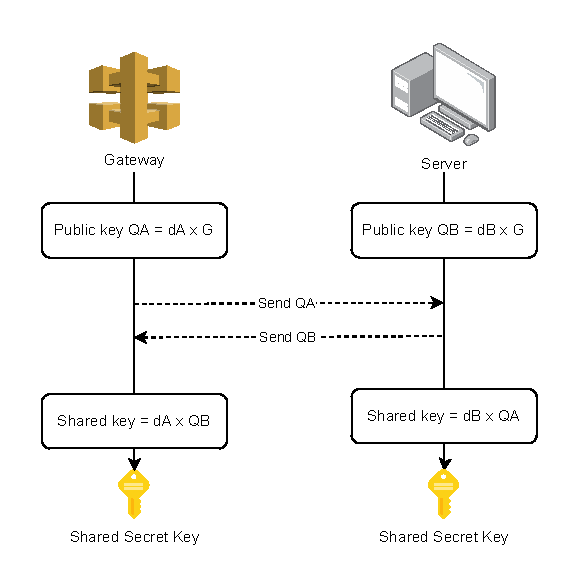
\includegraphics[width=0.65\linewidth]{images/keyexchange.pdf}
    \caption{Quá trình thực hiện trao đổi khóa ECDH}
    \label{fig:curve}
\end{figure}

Đề tài sử dụng đường cong \textit{sect163k1} trên trường hữu hạn $GF(2^{163})$, có phương trình sau:
\[
f(x) = x^{163} + x^7 + x^6 + x^3 + 1,
\]
được SECG (Standards for Efficient Cryptography Group) đề xuất nhờ khả năng tính toán hiệu quả trong họ đường cong Koblitz, giúp giảm chi phí xử lý tính toán. Với mức độ bảo mật tương đương 80-bit, đường cong này phù hợp cho các thiết bị IoT có tài nguyên hạn chế trong việc trao đổi khóa bảo mật \cite{secg}. Các tham số quan trọng bao gồm:

\[
a = 1, \quad b = 1, \quad h = 2,
\]
\[
n = \mathtt{04\; 00000000\; 00000000\; 00020108\; a2e0cc0d\; 99f8a5ef},
\]
Với điểm cơ sở \(G\):
\[
\begin{aligned}
G_x &= \mathtt{00000002\; fe13c053\; 7bbc11ac\; aa07d793} \\
    &\quad \mathtt{de4e6d5e\; 5c94eee8} \\
G_y &= \mathtt{00000002\; 89070fb0\; 5d38ff58\; 321f2e80} \\
    &\quad \mathtt{0536d538\; ccdaa3d9}
\end{aligned}
\]

ECDH đã được chứng minh có độ an toàn tương đương với thuật toán Diffie-Hellman truyền thống nhưng sử dụng các khóa có kích thước nhỏ hơn nhiều \cite{?} được trình bày ở Bảng \ref{tab:dh_ec_security}, điều này đặc biệt phù hợp với các thiết bị IoT có hạn chế về tài nguyên xử lý và bộ nhớ.

\begin{table}[h]
\centering
\small
\caption{Ratio of DH Security to EC Security at Different Security Levels}
\label{tab:dh_ec_security}
\begin{tabular}{|c|c|}
\hline
\textbf{Security Level (bits)} & \textbf{Ratio (DH : EC)} \\
\hline
80  & 3 : 1  \\
\hline
112 & 6 : 1  \\
\hline
128 & 10 : 1 \\
\hline
192 & 32 : 1 \\
\hline
256 & 64 : 1 \\
\hline
\end{tabular}
\end{table}

Mặc dù ECDH đòi hỏi chi phí tính toán cao hơn so với một số phương pháp đơn giản khác như sử dụng timestamp, bộ đếm (counter) hoặc khóa tĩnh, việc lựa chọn đường cong elliptic phù hợp sẽ giúp cân bằng giữa hiệu suất và bảo mật, từ đó đảm bảo hệ thống duy trì được mức độ an toàn trong thời gian dài.

\subsection{Hàm băm nhẹ ASCON}
\label{sec:ascon-hash}
Ascon sử dụng cấu trúc sponge duplex để cung cấp cả chức năng băm mật mã và mã hóa xác thực. Cấu trúc sponge là một phương thức vận hành, ánh xạ dữ liệu đầu vào có độ dài bất kỳ sang đầu ra có độ dài tuỳ chỉnh, thông qua một hàm hoán vị cố định và quy tắc đệm (padding). Cấu trúc này hoạt động trên một trạng thái hữu hạn, lặp lại việc áp dụng hàm hoán vị nội bộ, tổng quát hóa cả mã dòng với đầu vào cố định và hàm băm với đầu ra cố định. Sponge duplex là một biến thể của sponge, cho phép xen kẽ các khối đầu vào và đầu ra với tốc độ tương đương \cite{Ascon-Hash}.

Ascon-Hash là một hàm băm nhẹ, thực hiện hoán vị trên dữ liệu có kích thước bất kỳ để tạo ra giá trị băm 256-bit cố định, tối ưu cho các thiết bị nhúng. Hàm này sử dụng các thao tác đơn giản như XOR, dịch vòng (rotation), AND, NOT cùng với các hằng số để tối ưu hóa lớp thay thế (substitution layer), giúp giảm diện tích phần cứng và tiết kiệm tài nguyên \cite{Ascon-Hash}. Đặc tính nhẹ của Ascon-Hash cho phép triển khai hiệu quả trên các thiết bị IoT tài nguyên thấp, hỗ trợ nhiều bộ xử lý trong hệ thống với chi phí thấp.
Dựa trên cấu trúc sponge, Ascon-Hash vận hành qua hai giai đoạn chính: 
\begin{enumerate}
    \item Hấp thụ (Absorption): Dữ liệu đầu vào được chia thành các khối 64-bit, mỗi khối được XOR với trạng thái nội bộ 320-bit, sau đó áp dụng hàm hoán vị 12 vòng với các thao tác Addition, Rotation, XOR.
    \item Nén (Squeezing): Sau khi hấp thụ, trạng thái được xử lý thêm 12 vòng để tạo giá trị băm cuối cùng. 
\end{enumerate}
Ở mỗi phiên, khóa bí mật được tạo ra sau khi thực hiện trao đổi khóa ECDH sẽ được đưa vào hàm Ascon-Hash nhằm tạo ra khóa phiên cho mã hóa và giải mã dữ liệu.
% \subsection{Kiến trúc khung truyền}
% (có thể thêm để nói về kiến trúc khung truyền)

\section{Phương pháp thực hiện}
\label{sec:phuongphap}
\subsection{Tổng quan hệ thống IoT}
Mô hình IoT được triển khai dựa trên kiến trúc IoT bốn lớp như trình bày ở phần \ref{sec:4layer}. Ở lớp nhận thức, vi điều khiển STM32F411VET6 được sử dụng để thu thập dữ liệu từ cảm biến. Dữ liệu sau đó được truyền tới lớp xử lý dữ liệu thông qua ESP32, thiết bị đóng vai trò như một gateway trung gian. Giao tiếp giữa STM32 và ESP32 được thực hiện thông qua giao thức UART. Trên máy chủ Linux, các thành phần được triển khai bao gồm MQTT Broker và Backend chịu trách nhiệm tiếp nhận dữ liệu từ gateway, xử lý và phân giải các gói tin, kiểm tra tính hợp lệ của gói tin. Hình \ref{fig:realsystem} trình bày mô hình tổng quan của hệ thống. Phần dưới đây sẽ trình bày từng thành phần trong hệ thống, các khái niệm về khung truyền được đề cập tới sẽ trình bày chi tiết ở các phần \ref{sec:tongquan} và \ref{sec:frame}.

 % MQTT Broker đảm nhiệm việc thiết lập và duy trì kênh giao tiếp theo giao thức MQTT giữa gateway và máy chủ. Trong khi đó, Backend thực hiện xử lý nội dung dữ liệu, giải mã thông tin và quản lý cơ chế trao đổi khóa bảo mật với gateway. Những gói tin không hợp lệ sẽ được Backend Server phát hiện và từ chối ngay lập tức nhằm đảm bảo tính ổn định và an toàn cho người dùng cuối. 

\begin{figure}[h]
    \centering
    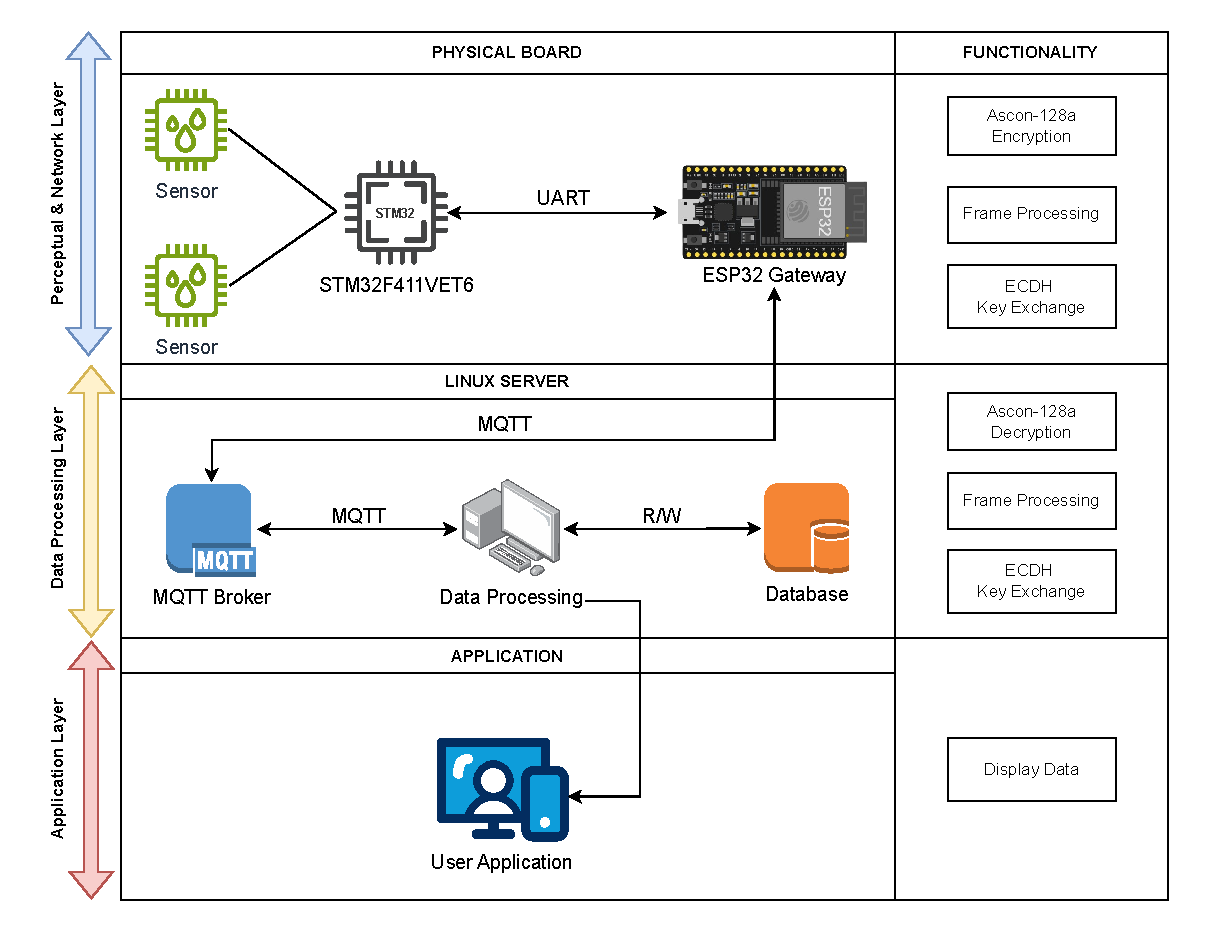
\includegraphics[width=1\linewidth]{realsystem.pdf}
    \caption{Mô hình tổng quan hệ thống}
    \label{fig:realsystem}
\end{figure}

\subsubsection{STM32F411VET6 MCU}
Vi điều khiển STM32F411VET6 được phát triển dựa trên bộ công cụ STM32CubeIDE kết hợp với STM32CubeMX. Trong kiến trúc hệ thống đề xuất, STM32 được sử dụng ở lớp nhận thức nhằm thu thập dữ liệu xung quanh thông qua các cảm biến được kết nối. Sau khi dữ liệu được thu thập, STM32 sẽ tiến hành mã hóa dữ liệu bằng thuật toán mã hóa nhẹ Ascon-128a. Tiếp theo, STM32 sẽ cấu trúc dữ liệu đã mã hóa thành khung truyền, và gửi đến lớp mạng để tiếp tục xử lý. Trước mỗi lần mã hóa, STM32 sẽ tạo các khóa phiên bằng cách sử dụng hàm băm Ascon Hash, đảm bảo mỗi khối dữ liệu sẽ sử dụng một khóa mã hóa khác nhau nhằm tăng cường tính bảo mật (kỹ thuật tạo khóa phiên sẽ được trình bày ở phần \ref{sec:key}). Thứ tự khóa phiên sẽ được STM32 đồng bộ liên tục cùng với máy chủ để đảm bảo quá trình mã hóa - giải mã được thực hiện chính xác.

\subsubsection{ESP32 Gateway}
ESP32 đóng vai trò như một IoT gateway tại lớp mạng trong mô hình IoT bốn lớp. Đây là thành phần quan trọng và có mức độ phức tạp cao nhất trong quá trình triển khai hệ thống. ESP32 đóng vai trò trung gian, thực hiện chuyển tiếp dữ liệu giữa lớp nhận thức (các thiết bị cảm biến sử dụng vi điều khiển STM32) sử dụng giao thức UART và lớp xử lý dữ liệu (máy chủ) sử dụng giao thức MQTT. Mọi khung truyền được gửi đến gateway sẽ được phân giải và kiểm tra tính toàn vẹn trước khi chuyển tiếp giữa các lớp, đảm bảo rằng chỉ dữ liệu hợp lệ mới được truyền đi. ESP32 là thiết bị thực hiện việc cấu trúc nhiều bộ khung truyền nhất trong hệ thống với tổng cộng năm bộ khung được định nghĩa và sử dụng tại đây. ESP32 cũng là nơi bắt đầu quá trình trao đổi khóa bí mật chung, khi khóa bí mật chung hết hạn hoặc có dấu hiện bị lộ, ESP32 sẽ tiến hành yêu cầu quá trình trao đổi khóa bí mật chung với máy chủ. Đặc biệt, cơ chế \textit{safe counter} (trình bày ở phần \ref{sec:safe_counter}) cũng được triển khai trong ESP32, đây là một trong những cơ chế quan trọng giúp tăng tính bảo mật của hệ thống. Nhìn chung, đây là thành phần rất quan trọng, không chỉ đảm nhận chức năng giao tiếp mà còn thực hiện nhiều nhiệm vụ bảo mật quan trọng, góp phần đảm bảo sự ổn định và an toàn của toàn bộ kiến trúc IoT.

\subsubsection{Hệ thống máy chủ}
Máy chủ đóng vai trò trung tâm trong hệ thống IoT nằm ở lớp xử lý dữ liệu trong kiến trúc IoT bốn lớp, chịu trách nhiệm tiếp nhận dữ liệu từ gateway, xử lý và phân giải các gói tin, kiểm tra tính hợp lệ của gói tin, sau đó cung cấp thông tin đến người dùng cuối. Trong hệ thống này, thành phần máy chủ được triển khai trên máy tính sử dụng hệ điều hành Linux. Trên máy chủ bao gồm hai thành phần chính là hệ thống Backend và MQTT Broker. 

Đầu tiên là thành phần MQTT Broker, được triển khai trên máy chủ sử dụng Aedes. Đây là một MQTT Broker nhẹ được phát triển bằng ngôn ngữ JavaScript, phù hợp để tích hợp với hệ thống Node.js. Việc lựa chọn tự triển khai MQTT Broker trên máy chủ thay vì sử dụng các dịch vụ MQTT Broker public xuất phát từ hai lý do chính. Trước hết, độ trễ khi sử dụng Broker public thường cao hơn nhiều do lượng lớn người dùng chia sẻ cùng một hạ tầng dẫn đến tình trạng tắc nghẽn hoặc chậm phản hồi. Ngược lại, triển khai Broker riêng giúp tối ưu tốc độ giao tiếp nhờ kiểm soát hoàn toàn tài nguyên và môi trường mạng. Thứ hai, tự cấu hình Broker cho phép tích hợp thêm các tính năng bảo mật quan trọng như xác thực người dùng, phân quyền truy cập theo topic, và giới hạn quyền publish/subscribe chỉ dành cho các thiết bị đáng tin cậy. Điều này nâng cao tính bảo mật và khả năng kiểm soát trong hệ thống, đặc biệt quan trọng đối với các ứng dụng IoT yêu cầu tính riêng tư và độ tin cậy cao. 

Hệ thống Backend chính là nơi tiếp nhận dữ liệu từ gateway và tiến hành xử lý dữ liệu. Khi nhận được khung truyền từ gateway, Backend sẽ tiến hành phân giải để kiểm tra, đối với các gói tin không hợp lệ, Backend có khả năng từ chối ngay lập tức để không ảnh hưởng đến người dùng. Trong kiến trúc hệ thống này, Backend được cấu hình để thực hiện một số chức năng quan trọng liên quan đến bảo mật và xử lý dữ liệu. Thuật toán trao đổi khóa ECDH được sử dụng để thiết lập khóa chung bí mật giữa gateway, trong khi thuật toán Ascon-128a đảm nhiệm việc giải mã và xác thực dữ liệu nhận được. Ngoài ra, máy chủ còn sử dụng hàm băm Ascon Hash nhằm tạo ra khóa phiên cho quá trình giải mã. Cơ chế \textit{safe counter} cũng được triển khai tại đây nhằm tăng tính bảo mật của hệ thống. Hệ thống Backend được triển khai trên nền tảng Node.js, với JavaScript là ngôn ngữ lập trình chính, giúp đảm bảo khả năng mở rộng, xử lý bất đồng bộ hiệu quả và dễ dàng tích hợp với các thành phần khác trong hệ thống.


\subsection{Mô hình giao tiếp của hệ thống}
\label{sec:tongquan}
Hệ thống IoT được chia thành ba quá trình giao tiếp: khởi tạo, trao đổi khóa và truyền dữ liệu. Tất cả dữ liệu trên đường truyền được đảm bảo mã hóa và xác thực. Ngoài ra, tất cả quá trình truyền sẽ được đóng gói thành các khung truyền được cấu hình độc nhất cho mỗi gói tin trình bày ở phần \ref{sec:4layer}. Hình \ref{fig:system} minh họa mô hình giao tiếp của hệ thống.

\begin{figure}[h]
    \centering
    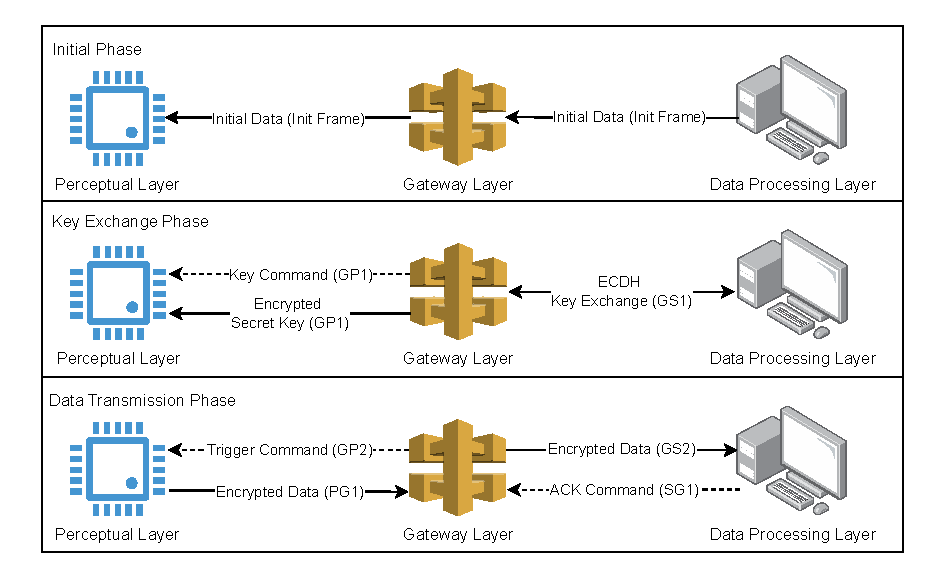
\includegraphics[width=0.85\linewidth]{images/system.pdf}
    \caption{Mô hình giao tiếp của hệ thống}
    \label{fig:system}
\end{figure}

Mỗi khi thiết bị khởi động hoặc reboot, phiên khởi tạo sẽ được kích hoạt. Trong phiên này, máy chủ sẽ truyền các thông tin đồng bộ, bao gồm \textit{safe counter} và \textit{key index} đến thiết bị. Những dữ liệu này đóng vai trò thiết yếu trong việc đảm bảo đồng bộ hóa, khôi phục trạng thái hệ thống, và duy trì tính toàn vẹn của quá trình truyền dữ liệu. Phần \ref{sec:safe_counter} sẽ trình bày ý nghĩa của \textit{safe counter} và phần \ref{sec:key} sẽ trình bày chi tiết về cách hoạt động của \textit{key index}.

Trong quá trình trao đổi khóa, gateway và máy chủ sẽ trao đổi khóa với nhau bằng thuật toán ECDH để có thể tạo ra hai khóa bí mật sử dụng cho mã hóa và giải mã. Dữ liệu sẽ được mã hóa ngay tại lớp nhận thức, vì vậy sau khi sinh thành công khóa bí mật, gateway sẽ chuyển khóa này đến lớp giao thức để tiến hành mã hóa dữ liệu. Để tránh lộ khóa bí mật, gateway tiến hành mã hóa khóa này bằng một khóa chia sẻ trước (pre-shared key) trước khi truyền xuống lớp nhận thức. Tại lớp nhận thức, khóa được giải mã và sử dụng cho quá trình mã hóa dữ liệu. Cơ chế này giúp đảm bảo khóa bí mật không bị lộ hoặc đánh chặn trong quá trình trao đổi khóa, qua đó tăng cường tính an toàn cho hệ thống.

Phần lớn thời gian STM32 tại lớp nhận thức sẽ ở trong chế độ ngủ (Sleep Mode) để có thể tiết kiệm năng lương, vì vậy để bắt đầu quá trình truyền dữ liệu, gateway trước tiên sẽ gửi một tín hiệu kích hoạt (trigger signal) cho lớp nhận thức. Khi nhận được tín hiệu, lớp nhận thức sẽ thoát khỏi sleep mode để tiến hành thu thập và mã hóa dữ liệu thu được bằng các khóa phiên được băm từ khóa bí mật (như trình bày ở phần \ref{sec:ascon-hash}) và gửi lên cho gateway. Gateway sẽ tiếp tục chuyển tiếp dữ liệu này lên cho máy chủ để xử lý. Nếu máy chủ có thể giải mã dữ liệu thành công, máy chủ sẽ gửi lại cho gateway một tín hiệu ACK nhằm thông báo phiên truyền dữ liệu thành công và tiếp tục bắt đầu phiên truyền mới. Trong trường hợp gateway không nhận được tín hiệu ACK từ máy chủ sau một khoảng thời gian nhất định (timeout), điều này có nghĩa dữ liệu đã không được truyền thành công hoặc giải mã không thành công, gateway sẽ gửi một gói tin thông báo cho STM32 ở lớp nhận thức để STM32 đồng bộ lại dữ liệu và bắt đầu lại phiên truyền. Hình \ref{fig:trans-sys} mô tả chi tiết toàn bộ quá trình giao tiếp của hệ thống bao gồm các khung truyền sẽ được trình bày chi tiết trong phần \ref{sec:frame}.

\begin{figure}[htbp]
    \centering
    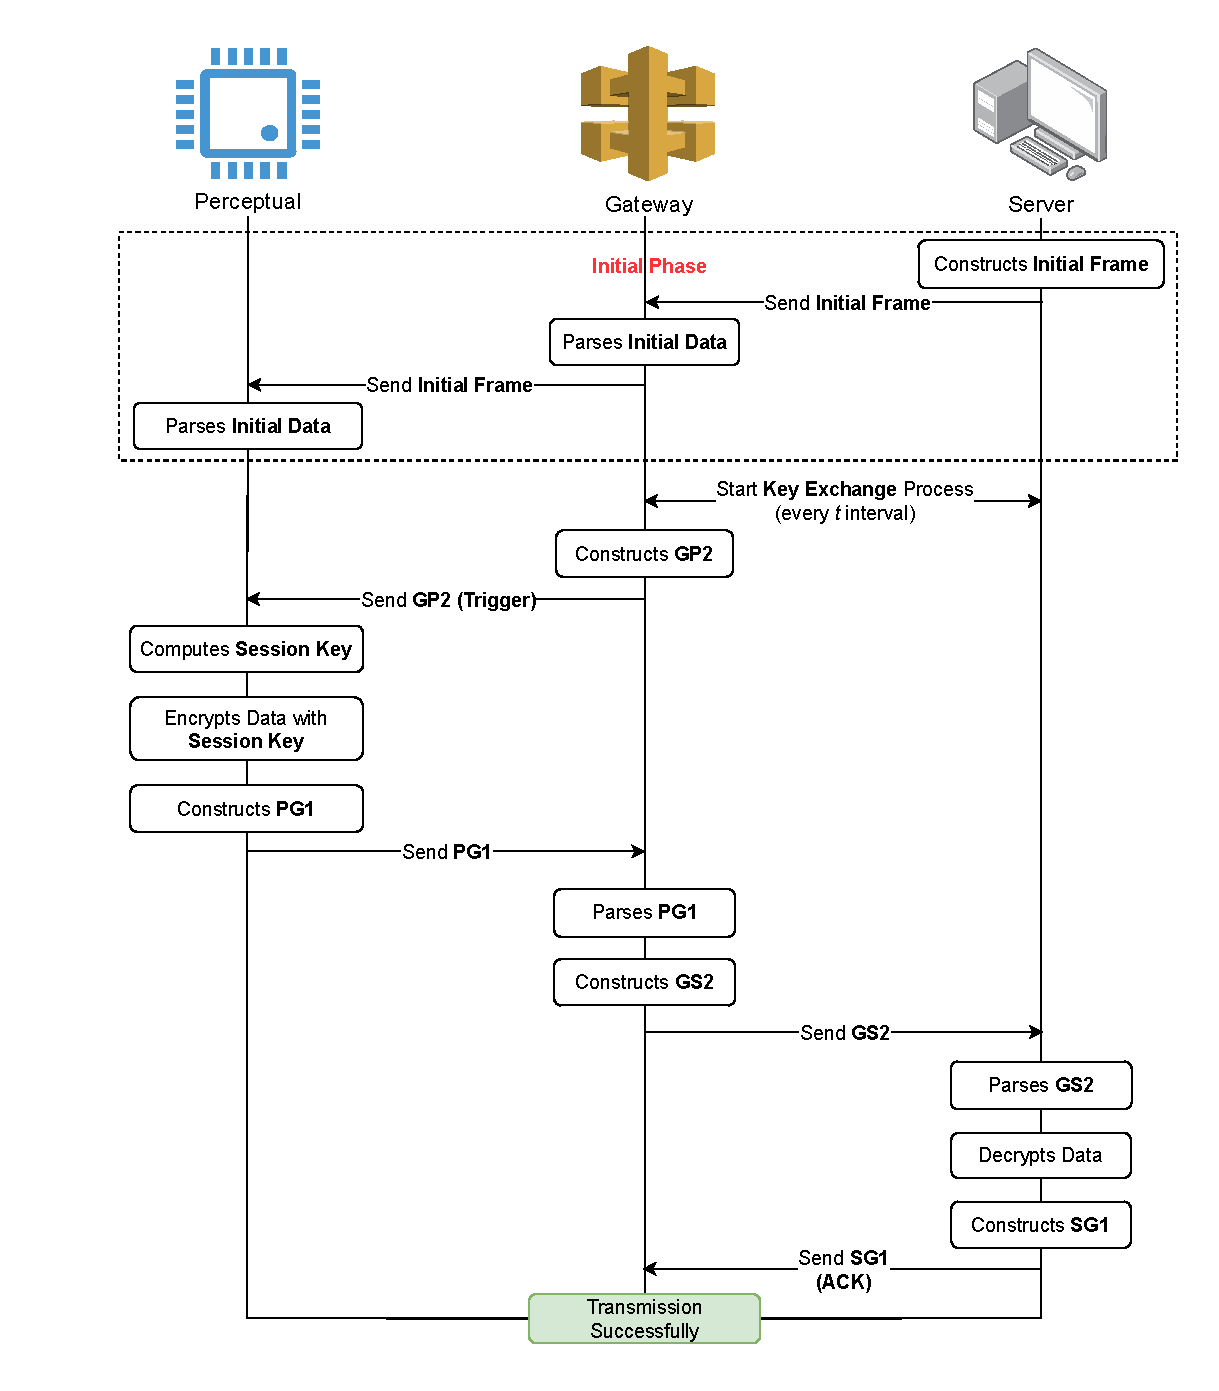
\includegraphics[width=1\linewidth]{trans-sys.pdf}
    \caption{Luồng hoạt động của hệ thống}
    \label{fig:trans-sys}
\end{figure}

\subsection{Phương pháp tạo khóa phiên từ khóa bí mật sử dụng trong mã hóa và giải mã dữ liệu}
\label{sec:key}
Để đảm bảo an toàn cho hệ thống IoT, việc thiết kế một phương thức trao đổi khóa bí mật an toàn là vô cùng cần thiết. Khóa bí mật này đóng vai trò quan trọng trong việc mã hóa và giải mã dữ liệu, góp phần bảo vệ tính toàn vẹn và bảo mật thông tin truyền tải. Nếu hệ thống IoT sử dụng phương pháp trao đổi khóa, tạo khóa kém an toàn hoặc dựa trên khóa tĩnh được cài đặt một lần duy nhất, nguy cơ lộ khóa hoặc bị tấn công brute-force với khóa có độ dài bit bảo mật thấp sẽ tăng lên đáng kể. 

Như đã trình bày trong phần \ref{sec:ecdh}, nhược điểm lớn của ECDH chính là chi phí tính toán lớn, điều này có thể ảnh hưởng đến độ trễ của hệ thống. Vì vậy, để đảm bảo khóa luôn được làm mới và hạn chế quá trình trao đổi khóa liên tục, đề tài đề xuất một phương pháp tạo khóa phiên dựa trên khóa bí mật để giải quyết vấn đề trên. Trong đề tài này, thuật toán trao đổi khóa Elliptic Curve Diffie-Hellman (ECDH) được áp dụng nhằm thiết lập khóa bí mật trên kênh truyền không an toàn, đồng thời kết hợp với hàm băm nhẹ ASCON để sinh các khóa phiên (session key) phục vụ cho quá trình mã hóa, giải mã dữ liệu. Hình \ref{fig:skey} thể hiện quá trình tạo khóa phiên đề xuất.

\begin{figure}[h]
    \centering
    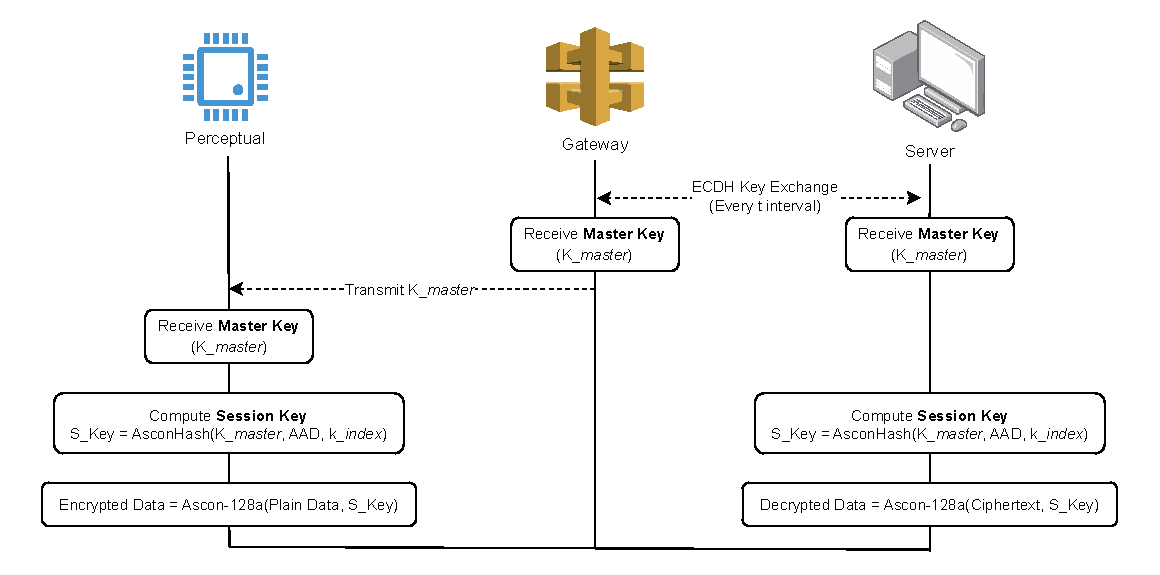
\includegraphics[width=1\linewidth]{skey.pdf}
    \caption{Quy trình tạo khóa phiên}
    \label{fig:skey}
\end{figure}

Sau khi hoàn thành trao đổi khóa như đã trình bày ở phần \ref{sec:ecdh}, gateway và server sẽ tạo ra hai khóa bí mật, ở phần này sẽ gọi là Master Key ($K_{master}$). Thời gian giữa mỗi lần trao đổi $K_{master}$ được gọi là $t$, được cấu hình tùy vào yêu cầu bảo mật của hệ thống, $t$ càng nhỏ thì quá trình trao đổi $K_{master}$ sẽ diễn ra với tần suất nhiều hơn nhưng bù lại sẽ tốn nhiều tài nguyên và thời gian cho việc trao đổi khóa. Và như đã trình bày ở phần \ref{sec:tongquan}, $K_{master}$ sẽ được truyền xuống lớp nhận thức để phục vụ quá trình mã hóa.  Trước khi lớp nhận thức mã hóa dữ liệu, khóa phiên sẽ được tạo ra bằng hàm băm ASCON. Đầu vào của hàm băm ASCON là sự kết hợp của các thành phần sau: $K_{master}$, $AAD$ và $k_{index}$. Trong đó $AAD$ là Associated Data được sử dụng trong mã hóa xác thực Ascon-128a và $k_{index}$ chính là thứ tự của khóa hiện tại và tăng dần sau mỗi phiên. 
\[
input = K_{master} || \text{AAD} ||k_{index}
\]
Kết quả của hàm băm với đầu vào $input$ sẽ cho ra khóa phiên và sử dụng cho việc mã hóa dữ liệu. Phía server cũng sẽ sử dụng quá trình tương tự để tạo khóa phiên cho việc giải mã. Với $k_{index}$ thay đổi liên tục, khóa phiên sinh ra cũng sẽ thay đổi liên tục, đảm bảo việc dò khóa sẽ rất phức tạp. 

\[
    K_{session} = \text{AsconHash}(K_{master} || \text{AAD} ||k_{index})
\]

\subsection{Kiến trúc khung truyền giao tiếp giữa các lớp trong hệ thống IoT}
\label{sec:frame}
Phần này sẽ trình bày chi tiết về kiến trúc khung truyền được sử dụng trong hệ thống, được sử dụng trong giao tiếp giữa các lớp như minh họa ở hình \ref{fig:system}. Tất cả các khung đều có định dạng chung được gọi là trường chuẩn, khởi đầu với 2-byte \textit{Start of Frame} (SOF) để một phiên truyền. Tiếp theo đó sẽ là 4-byte \textit{Identifier ID}, định danh thiết bị truyền dữ liệu, \textit{ID} này sẽ được cấu hình tĩnh bên trong thiết bị ở lớp nhận thức. Khung truyền sẽ kết thúc bằng 2-byte \textit{End of Frame} (EOF). Trường chứa dữ liệu (\textit{Data field}) của khung truyền sẽ thay đổi tùy theo mục đích của quá trình truyền, ví dụ trường dữ liệu của khung truyền trao đổi khóa sẽ khác với trường dữ liệu của khung truyền dữ liệu mã hóa. Ngoài các trường chuẩn ở trên, mỗi khung truyền sẽ có thêm một số trường bổ sung để tăng cường độ bảo mật và tin cậy của hệ thống. 

Để dễ hiểu, mỗi khung truyền sẽ được đặt tên dựa trên lớp nguồn và lớp đích, ngoại trừ khung truyền khởi tạo; ví dụ, một khung truyền từ gateway đến máy chủ (server) sẽ được ký hiệu là GS (Gateway-Server). Đối với dữ liệu liên quan (Associated Data - $AAD$), ở phần này sẽ sử dụng hai $AAD$ bao gồm $AAD_{data}$ và $AAD_{key}$. Trong đó, $AAD_{data}$ được tính toán mỗi phiên truyền dữ liệu và $AAD_{key}$ được cấu hình sẵn và sử dụng trong các phiên trao đổi khóa giữa gateway và máy chủ. Phần này sẽ chia các khung truyền thành ba nhóm chính: khung truyền khởi tạo, khung truyền trong giao tiếp giữa lớp nhận thức và gateway, khung truyền trong giao tiếp giữa gateway và máy chủ.
\subsubsection{Khung truyền khởi tạo}
Khung truyền khởi tạo này có kiến trúc rất đơn giản, chỉ bao gồm các trường chuẩn như trình bày ở phần trên. Khung truyền này chứa các dữ liệu cần thiết giúp máy chủ đồng bộ giao tiếp với thiết bị. Trường dữ liệu của khung khởi tạo bao gồm 2-byte \textit{safe counter} và 2-byte \textit{key index} hỗ trợ thiết lập trạng thái ban đầu và đảm bảo tính toàn vẹn hệ thống. Trong suốt vòng đời hoạt động, khung khởi tạo chỉ được kích hoạt một lần duy nhất ngay sau khi thiết bị khởi động lại.
\begin{figure}[H]
    \centering
    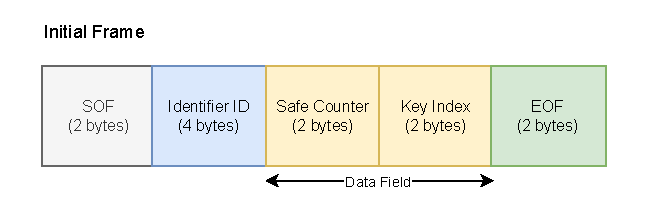
\includegraphics[width=0.6\linewidth]{init-frame.pdf}
    \caption{Khung truyền khởi tạo}
    \label{fig:init-frame}
\end{figure}
\subsubsection{Khung truyền trong giao tiếp giữa lớp nhận thức và lớp mạng}
Phần này mô tả chi tiết cấu trúc khung truyền trong quá trình giao tiếp giữa lớp nhận thức và lớp mạng. Hình \ref{fig:gp} minh họa khung truyền được sử dụng khi dữ liệu được gửi từ lớp mạng xuống lớp nhận thức, ký hiệu là GP. Trong khung truyền này, một trường 1 byte có tên là \textit{packet type} được thêm vào để xác định loại dữ liệu đang được truyền. Hai loại khung chính được định nghĩa: một dành cho việc truyền khóa bí mật (GP1), và một dành cho truyền tín hiệu kích hoạt (GP2). 

Với khung truyền GP2, trường dữ liệu của khung sẽ chỉ chứa 16-byte $AAD_{data}$ dùng cho mã hóa dữ liệu, tức là, lớp nhận thức sẽ sử dụng 16-byte $AAD_{data}$ này cho việc mã hóa dữ liệu trước khi truyền đi. Các trường chuẩn của GP2 vẫn được giữ nguyên.

Khung truyền GP1 sẽ có sự phức tạp hơn do đây là khung đảm nhận vai trò truyền khóa bí mật xuống lớp nhận thức, vì đây là dữ liệu nhạy cảm nên một số trường bổ sung được thêm vào. Trường dữ liệu của GP1 sẽ bao gồm 16-byte \textit{Nonce} và $AAD_{data}$, $AAD_{data}$ vẫn sẽ được sử dụng trong mã hóa dữ liệu trước khi truyền. \textit{Nonce} và $AAD_{key}$ là hai dữ liệu quan trọng để lớp nhận thức có thể giải mã khóa bí mật (khóa bí mật sẽ được mã hóa bởi gateway trước khi truyền xuống lớp nhận thức như trình bày ở phần \ref{sec:tongquan}) với $AAD_{key}$ đã được cấu hình tĩnh trước cho cả lớp giao thức và gateway. Tiếp theo đó, sẽ là 1-byte \textit{secret key length} và phần tải chứa khóa bí mật đã được mã hóa, trong đó 1-byte \textit{secret key length} biểu thị độ dài của khóa bí mật. Một trường quan trọng được bổ sung vào khung GP1 đó chính là 16-byte \textit{authentication tag} (Auth Tag), được sinh ra trong quá trình mã hóa khóa bí mật với Ascon-128a. Phần \ref{sec:mitm} đã trình bày việc tấn công Man-in-the-Middle có thể đánh tráo khóa trên đường truyền, vì vậy Auth Tag được thêm vào để đảm bảo dữ liệu được xác thực, nếu việc tính toán Auth Tag sai và không trùng khớp, lớp nhận thức sẽ ngay lập tức từ chối khóa bí mật này, tránh việc sử dụng khóa giả mạo cho việc mã hóa và giải mã.

Về cách tính $AAD_{data}$ trong GP1 và GP2, $AAD_{data}$ được ghép từ một số trường dữ liệu trong GS2 (trình bày ở phần \ref{sec:gs}). Vì thế, $AAD_{data}$ sẽ được tính như sau:
\[
\text{$AAD_{data}$} = \text{SOF}_{2} \, || \, \text{Identifier ID}_{4} \, || \, \text{Sequence Number}_{4} \, || \, \text{Nonce}_{4} \, || \, \text{EOF}_{2}
\]

\begin{figure}[h]
    \centering
    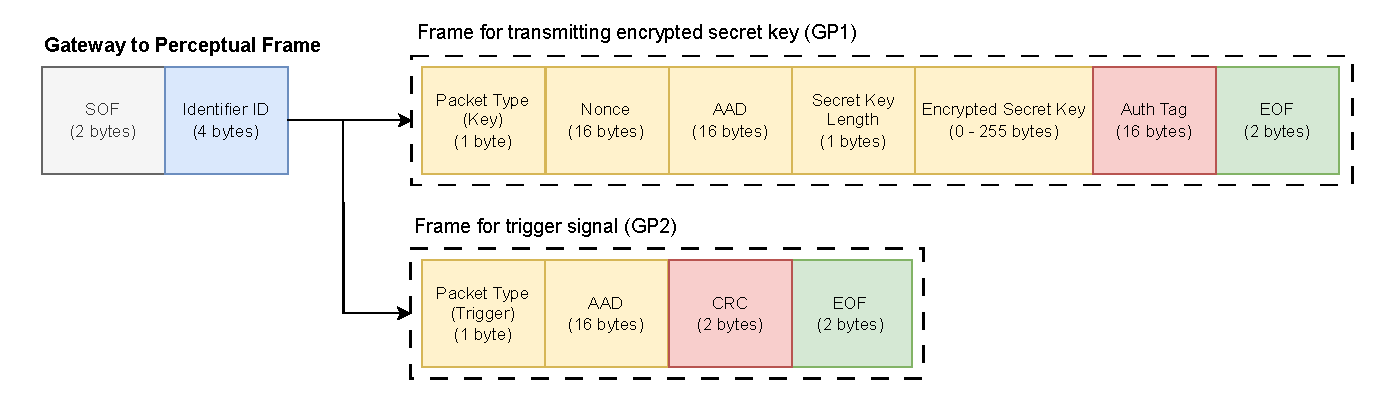
\includegraphics[width=1\linewidth]{gp-frame.pdf}
    \caption{Khung truyền trao truyền dữ liệu từ gateway xuống lớp nhận thức}
    \label{fig:gp}
\end{figure}

Khi nhận tín hiệu kích hoạt (khung GP2) từ gateway, lớp nhận thức sẽ tạo khung PG1 chứa dữ liệu mã hóa và gửi cho gateway (minh họa hình \ref{fig:pg-frame}). Trường dữ liệu của khung PG1 chứa 16-byte \textit{Nonce}, đây là \textit{Nonce} được dùng trong mã hóa dữ liệu và phía máy chủ sẽ dùng \textit{Nonce} này cho giải mã. Tiếp theo, 16-byte Auth Tag sẽ được gửi nhằm xác thực dữ liệu mã hóa, máy chủ sau khi giải mã sẽ so sánh Auth Tag, nếu có sự khác biệt về Auth Tag, máy chủ sẽ từ chối gói tin đó. Ngoài ra, 2-byte \textit{Cyclic Redundancy Check} (CRC) giúp phát hiện có sự sai lệch hay mất mác dữ liệu nào trong quá trình truyền.

\begin{figure}[H]
    \centering
    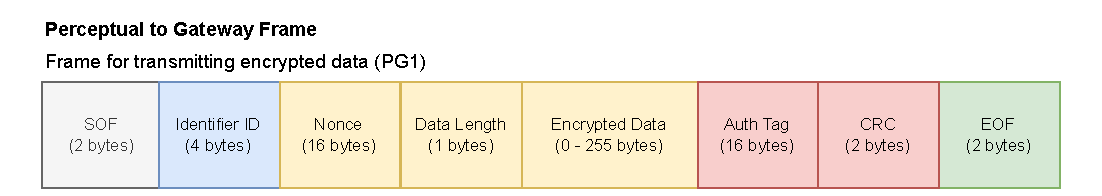
\includegraphics[width=0.9\linewidth]{pg-frame.pdf}
    \caption{Khung truyền trong truyền dữ liệu từ lớp nhận thức lên gateway}
    \label{fig:pg-frame}
\end{figure}

\subsubsection{Khung truyền trong giao tiếp giữa gateway và server}
\label{sec:gs}
Nhóm các khung truyền trong quá trình giao tiếp giữa gateway và máy chủ được minh họa trong Hình \ref{fig:gs-frame}. Tổng cộng có bốn loại khung truyền chính, bao gồm: GS1, GS2, SG1 và một khung truyền đặc biệt dùng để gửi thông tin trạng thái hiện tại của hệ thống lên máy chủ.

Khung truyền GS1 là khung được sử dụng để truyền thông tin về khóa công khai, phục vụ cho quá trình trao đổi khóa giữa gateway và máy chủ. Các trường chuẩn trong cấu trúc khung được giữ nguyên. Trường dữ liệu của khung chứa một \textit{Nonce} có độ dài 16 byte, dùng trong quá trình tính toán thẻ xác thực, tiếp đó là 1-byte \textit{public key length} và phần tải chứa khóa công khai. Do trường dữ liệu chứa thông tin quan trọng, việc bổ sung 16 byte Auth Tag giúp tăng cường bảo mật và hạn chế nguy cơ giả mạo khóa trong quá trình trao đổi. Auth Tag này được tạo ra bằng thuật toán Ascon-128a, sử dụng khóa chia sẻ trước cùng với giá trị $AAD_{key}$ đã được cấu hình sẵn giữa gateway và máy chủ. Để tối ưu hiệu suất tính toán, phần bản rõ (plaintext) được bỏ trống vì chỉ cần tạo Auth Tag. Điều này giúp giảm thời gian xử lý cho cả gateway và máy chủ, đồng thời vẫn đảm bảo tính toàn vẹn của khóa công khai. Sau khi nhận được khung GS1 từ gateway, máy chủ sẽ tiến hành kiểm tra các trường trong khung. Tiếp theo, máy chủ sử dụng thuật toán giải mã Ascon-128a với bản mã (ciphertext) rỗng, cùng với \textit{Nonce} và giá trị $AAD_{key}$ để tính lại Auth Tag. Auth Tag này sau đó được so sánh với Auth Tag nhận được nhằm xác minh tính toàn vẹn của thông tin khóa công khai. Hình \ref{fig:auth_t} minh họa việc tính toán Auth Tag trong quá trình trao đổi khóa.

\begin{figure}[h]
    \centering
    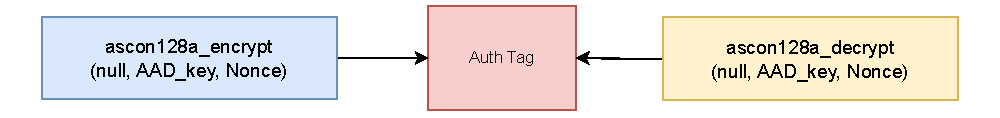
\includegraphics[width=0.85\linewidth]{auth_t.pdf}
    \caption{Tính toán thẻ xác thực (Auth Tag) trong trao đổi khóa}
    \label{fig:auth_t}
\end{figure}

Trong truyền dữ liệu mã hóa từ gateway lên máy chủ, khung truyền GS2 sẽ được sử dụng. Khung truyền này giữ lại các trường tương tự như GS1, tuy nhiên, GS2 được cấu hình thêm một trường 4-byte \textit{sequence number}. Khung truyền GS2 đóng vai trò chính trong quá trình truyền dữ liệu và được sử dụng thường xuyên trong suốt thời gian hệ thống hoạt động. Đây là loại khung được sử dụng phổ biến nhất, do đảm nhiệm chức năng truyền tải dữ liệu giữa gateway và máy chủ một cách liên tục và ổn định. Việc bổ sung 4 byte \textit{sequence number} vào khung truyền giúp tăng cường bảo mật trong quá trình truyền dữ liệu, nhằm ngăn chặn các cuộc tấn công như tấn công phát lại (replay attack) hoặc tấn công xen giữa (Man-in-the-Middle). Khi giải mã khung truyền, máy chủ sẽ kiểm tra sequence number hiện tại của gói tin. Nếu phát hiện bất kỳ sai lệch nào về giá trị này, gói tin sẽ bị từ chối ngay lập tức. Cơ chế này làm giảm nguy cơ tấn công phát lại, vì ngay cả khi kẻ tấn công thu được một gói tin cũ và cố gắng gửi lại, sequence number bên trong gói tin sẽ không còn phù hợp với trạng thái hiện tại, do giá trị này được tăng tuần tự qua từng phiên truyền. Trường dữ liệu của khung GS2 bao gồm một \textit{Nonce} có độ dài 16 byte, một trường \textit{payload length} dài 1 byte, phần tải chứa dữ liệu đã được mã hóa, và cuối cùng là Auth Tag dài 16 byte được tạo ra trong quá trình mã hóa dữ liệu. Các thành phần như Nonce, dữ liệu mã hóa và Auth Tag đều được trích xuất từ khung PG1 do lớp nhận thức gửi lên gateway. Khi máy chủ nhận được khung GS2, nó sẽ tách các trường cần thiết để tái tạo giá trị $AAD_{data}$, phục vụ cho quá trình giải mã và xác thực dữ liệu.

Khung SG1 được sử dụng như một tín hiệu điều khiển gửi từ máy chủ về gateway. Hiện tại, SG1 được cấu hình để phục vụ hai loại tín hiệu chính: tín hiệu xác nhận (ACK) nhằm thông báo rằng phiên truyền dữ liệu đã thành công, và tín hiệu cập nhật sequence number mới. Trong một số tình huống, khi máy chủ xác định cần cập nhật giá trị sequence number, nó sẽ sử dụng khung SG1 để gửi tín hiệu tương ứng đến gateway nhằm đảm bảo sự đồng bộ giữa hai bên.

Cuối cùng là một loại khung truyền đặc biệt, dùng để gửi các thông tin về tình trạng hoạt động của hệ thống, bao gồm các chỉ số như tỷ lệ chuyển gói thành công (PDR – Packet Delivery Ratio), độ trễ, số lượng gói tin đã truyền, và các thông số liên quan khác. Khung truyền này được gửi định kỳ lên máy chủ, thường mỗi vài phút một lần, nhằm cung cấp dữ liệu giám sát giúp người dùng theo dõi và đánh giá hiệu suất của hệ thống.

\begin{figure}
    \centering
    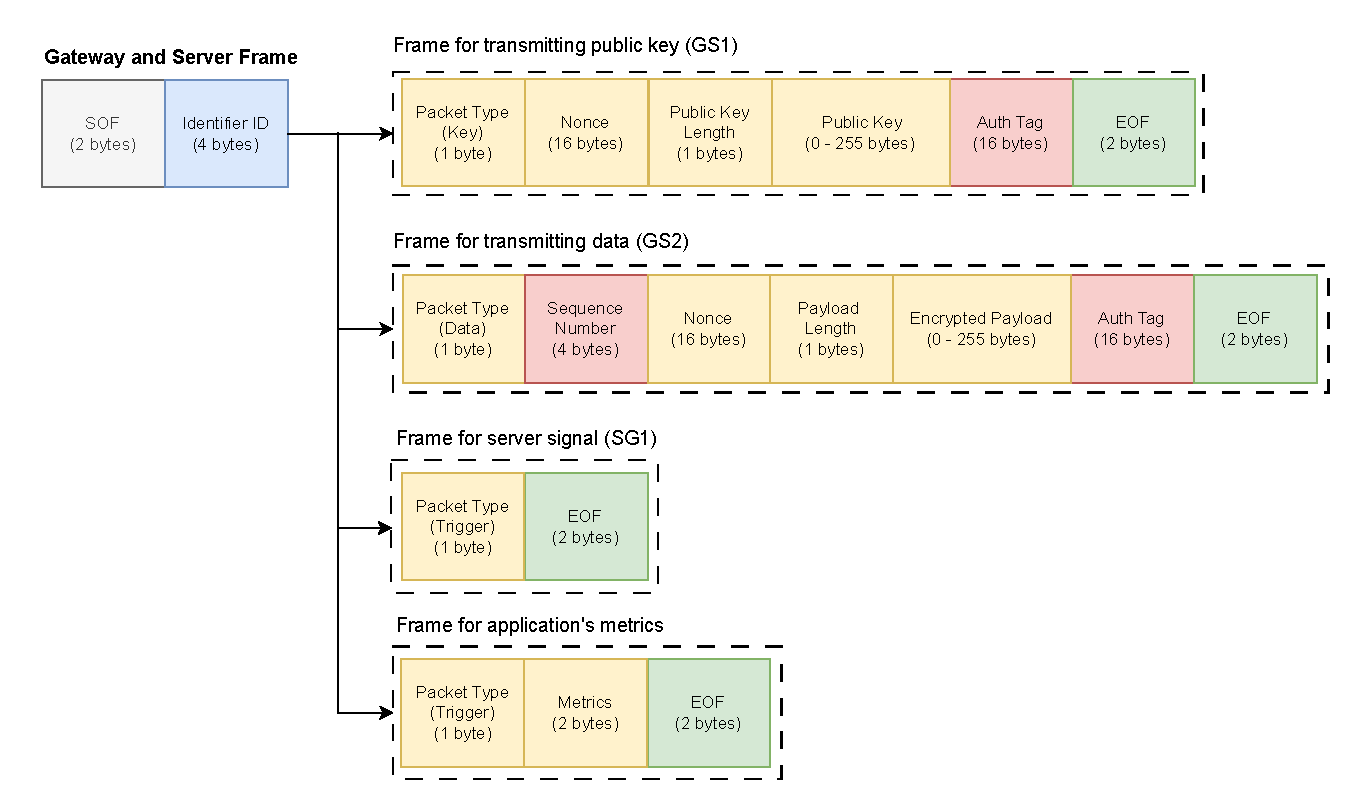
\includegraphics[width=1\linewidth]{gs-frame.pdf}
    \caption{Bộ khung truyền trong giao tiếp giữa gateway và máy chủ}
    \label{fig:gs-frame}
\end{figure}
\subsubsection{Quá trình phân giải khung truyền}
Quá trình phân giải khung truyền được trình bày trong hình \ref{fig:parsing} và \ref{fig:parse-function}. Tất cả các khung truyền được sử dụng trong hệ thống đều áp dụng chung quá trình phân giải này. Vì vậy, để đảm bảo tính ngắn gọn cũng như dễ hiểu trong báo cáo, khung truyền GS2 sẽ được minh họa trong hình để trình bày về quá trình phân giải khung truyền. Việc phân giải bắt đầu từ việc nhận dữ liệu từ thiết bị đích và lưu trữ vào trong một bộ đệm nội bộ (internal buffer), để chuẩn bị cho quá trình phân giải. Mỗi byte trong bộ đệm sẽ được luân phiên đưa vào hàm phân giải khung truyền (Hình \ref{fig:parse-function}). Trong mỗi hàm phân giải, các điều kiện ở mỗi trường trong khung truyền được cấu hình sẵn. Từ đó, hàm phân giải sẽ kiểm tra số byte tương ứng trong bộ đệm nội bộ với điều kiện; nếu điều kiện đúng, hàm phân giải sẽ tiến hành kiểm tra trường tiếp theo; ngược lại, sẽ ngừng quá trình phân giải và trả về mã lỗi. Nếu hàm phân giải có thể phân giải được tất cả các trường trong bộ đệm, quá trình phân giải sẽ hoàn tất. Việc mã hóa dữ liệu sẽ được diễn ra trong quá trình phân giải này, cụ thể là trong bước tính thẻ xác thực. Ở bước này, dữ liệu sẽ được mã hóa, từ đó sinh ra thẻ xác thực, sau đó so sánh với thẻ xác thực nhận được để kiểm tra tính toàn vẹn của dữ liệu. 

\begin{figure}[H]
    \centering
    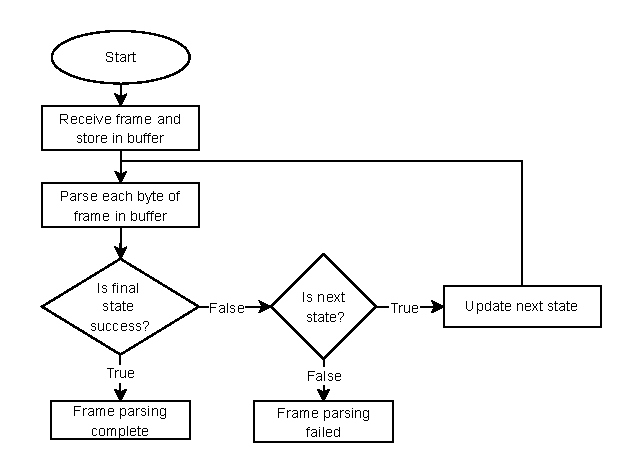
\includegraphics[width=0.7\linewidth]{frameparsing1.pdf}
    \caption{Quá trình phân giải khung truyền}
    \label{fig:parse-function}
\end{figure}

\begin{figure}[H]
    \centering
    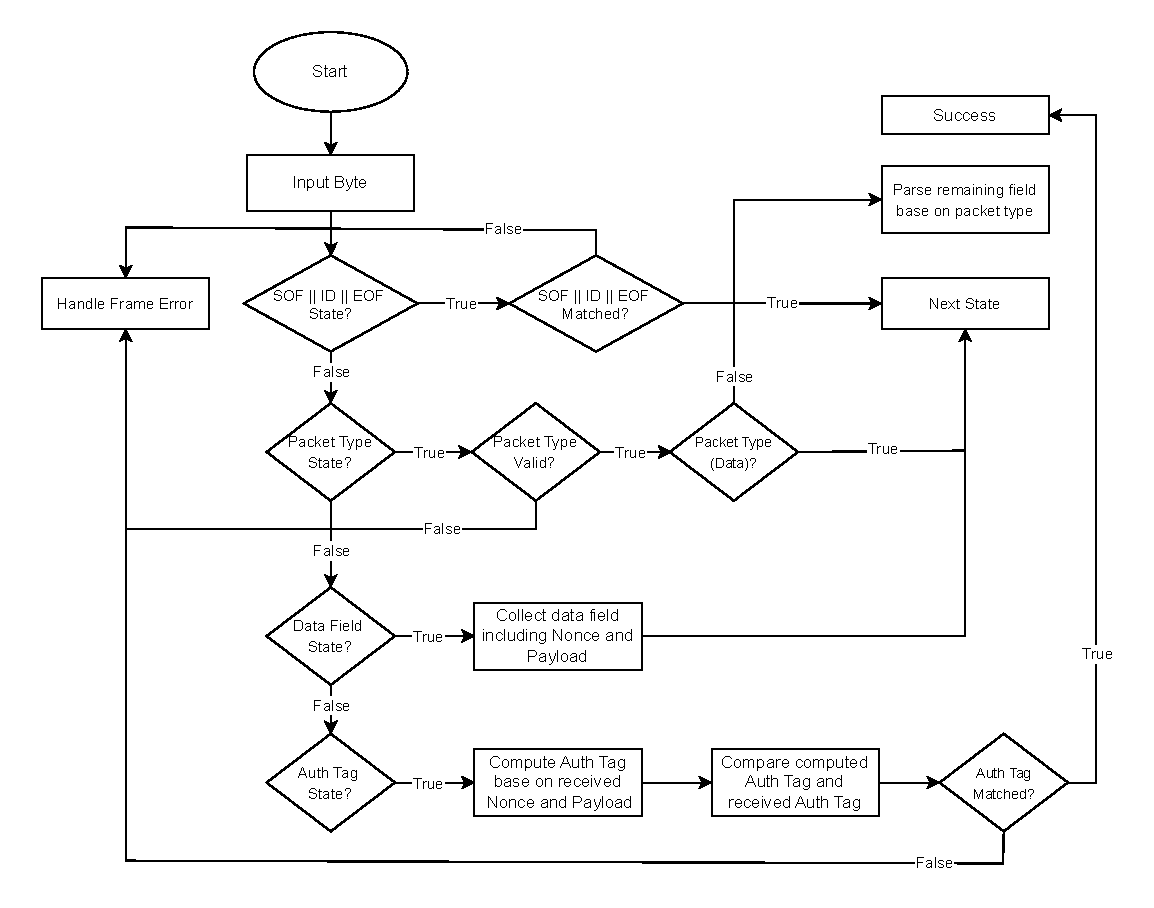
\includegraphics[width=1\linewidth]{frameparse.pdf}
    \caption{Hàm phân giải khung truyền GS2}
    \label{fig:parsing}
\end{figure}

\subsection{Cơ chế safe counter}
\label{sec:safe_counter}
Như đã đề cập ở phần \ref{sec:gs}, khung truyền GS2 được cấu hình thêm 4-byte \textit{sequence number} để hạn chế khả năng tấn công phát lại (replay attack) và tấn công xen giữa (Man-in-the-Middle). Tuy nhiên, một số trường hợp kẻ tấn công có thể gửi rất nhiều gói tin với các \textit{sequence number} khác nhau nhằm cố gắng brute-force thành công \textit{sequence number} hiện tại của hệ thống. Có thể thấy rằng với 4 byte \textit{sequence number}, sau khi toàn bộ không gian $2^{32}$ giá trị được thử, xác suất brute-force thành công sẽ đạt 100\%. Vấn đề đặt ra ở đây là xác suất thành công của brute-force tăng dần theo số lần thử — tức là bài toán mang tính xác suất tích lũy \cite{?}. Để khắc phục điều này, cơ chế safe counter được triển khai nhằm chuyển bài toán từ dạng có xác suất tăng dần thành một quá trình với xác suất thành công cố định ở mỗi lần thử, từ đó làm cho brute-force trở nên kém hiệu quả hơn. \textit{Safe counter} thực chất là một biến đếm 32-bit đồng bộ giữa gateway và máy chủ, biến đếm này sẽ được cập nhật liên tục trong quá trình truyền dữ liệu. Trong trường hợp bị brute-force, máy chủ sẽ từ chối các gói tin sai về \textit{sequence number} trong quá trình phân giải, số gói tin mà máy chủ từ chối sẽ được gọi là $R$. Ở máy chủ, một ngưỡng được đặt ra gọi là \(T_{\text{reject}} \), nếu máy chủ từ chối một số lượng gói tin chạm ngưỡng \(T_{\text{reject}} \), hay nói cách khác nếu $R \geq T_{reject}$, máy chủ sẽ ngay lập tức gửi một tín hiệu tới gateway bằng khung truyền SG1 và thực hiện việc cập nhật \textit{sequence number} mới dựa trên \textit{safe counter} hiện tại của hệ thống. Vì \textit{safe counter} được đồng bộ giữa gateway và máy chủ, việc tính toán lại \textit{sequence number} sẽ cho ra kết quả giống nhau, đảm bảo việc truyền dữ liệu giữa gateway và máy chủ vẫn diễn ra bình thường với \textit{sequence number} mới. Thuật toán \ref{alg:safe_counter} trình bày chi tiết cách tính \textit{sequence number} mới dựa trên \textit{safe counter}.

\begin{algorithm}[ht]
\caption{Cơ chế safe counter}
\small
\label{alg:safe_counter}
\begin{algorithmic}[1]
\Require 32-bit Safe Counter $SC$, Secret Key $K$, Threshold $T_{\text{rejected}}$, Rejected Packet Count $R$, Current Sequence Number $SN$
\State $SC \gets (SC + ((SC \ll 3) \oplus (SC \gg 2) \oplus 7)) \bmod 2^{32}$
\If{$R \geq T_{\text{rejected}}$}
    \State $SN \gets (SC \oplus K) \bmod 2^{32}$
    \State $R \gets 0$
\EndIf
\Return $SN$
\end{algorithmic}
\end{algorithm}

Với cơ chế này, kẻ tấn công sẽ có \(T_{\text{reject}} \) cơ hội để đoán trước khi \textit{sequence number} được cập nhật lại một giá trị mới ngẫu nhiên. Tỉ lệ đoán thành công \textit{sequence number} sau \(T_{\text{reject}} \) lần thử có công thức là:
\[
P_{\text{guess}} \approx 1 - \left(1 - \frac{1}{2^{32}}\right)^{T_{\text{rejected}}}.
\]
Trong hệ thống thử nghiệm, \(T_{\text{reject}} \) được đặt mặc định là 10, vì thế tỉ lệ cố định để có thể brute-force thành công \textit{sequence number} là:
\[
P_{\text{guess}} \approx 1 - \left(1 - \frac{1}{2^{32}}\right)^{10} \approx 0.00000023 \%
\]
Thử nghiệm trên 70,000 gói tin giả mạo với các \textit{sequence number} khác nhau được gửi vào hệ thống, kết quả cho thấy máy chủ từ chối hoàn toàn 70,000 gói tin, đạt tỉ lệ chính xác 100\%, cho thấy được độ tin cậy cao của cơ chế này. 

% Hình \ref{fig:sclog} trình bày quá trình cập nhật và đồng bộ \textit{sequence number} mới giữa gateway và máy chủ thông qua \textit{safe counter}:

% \begin{figure}[ht]
%     \centering
%     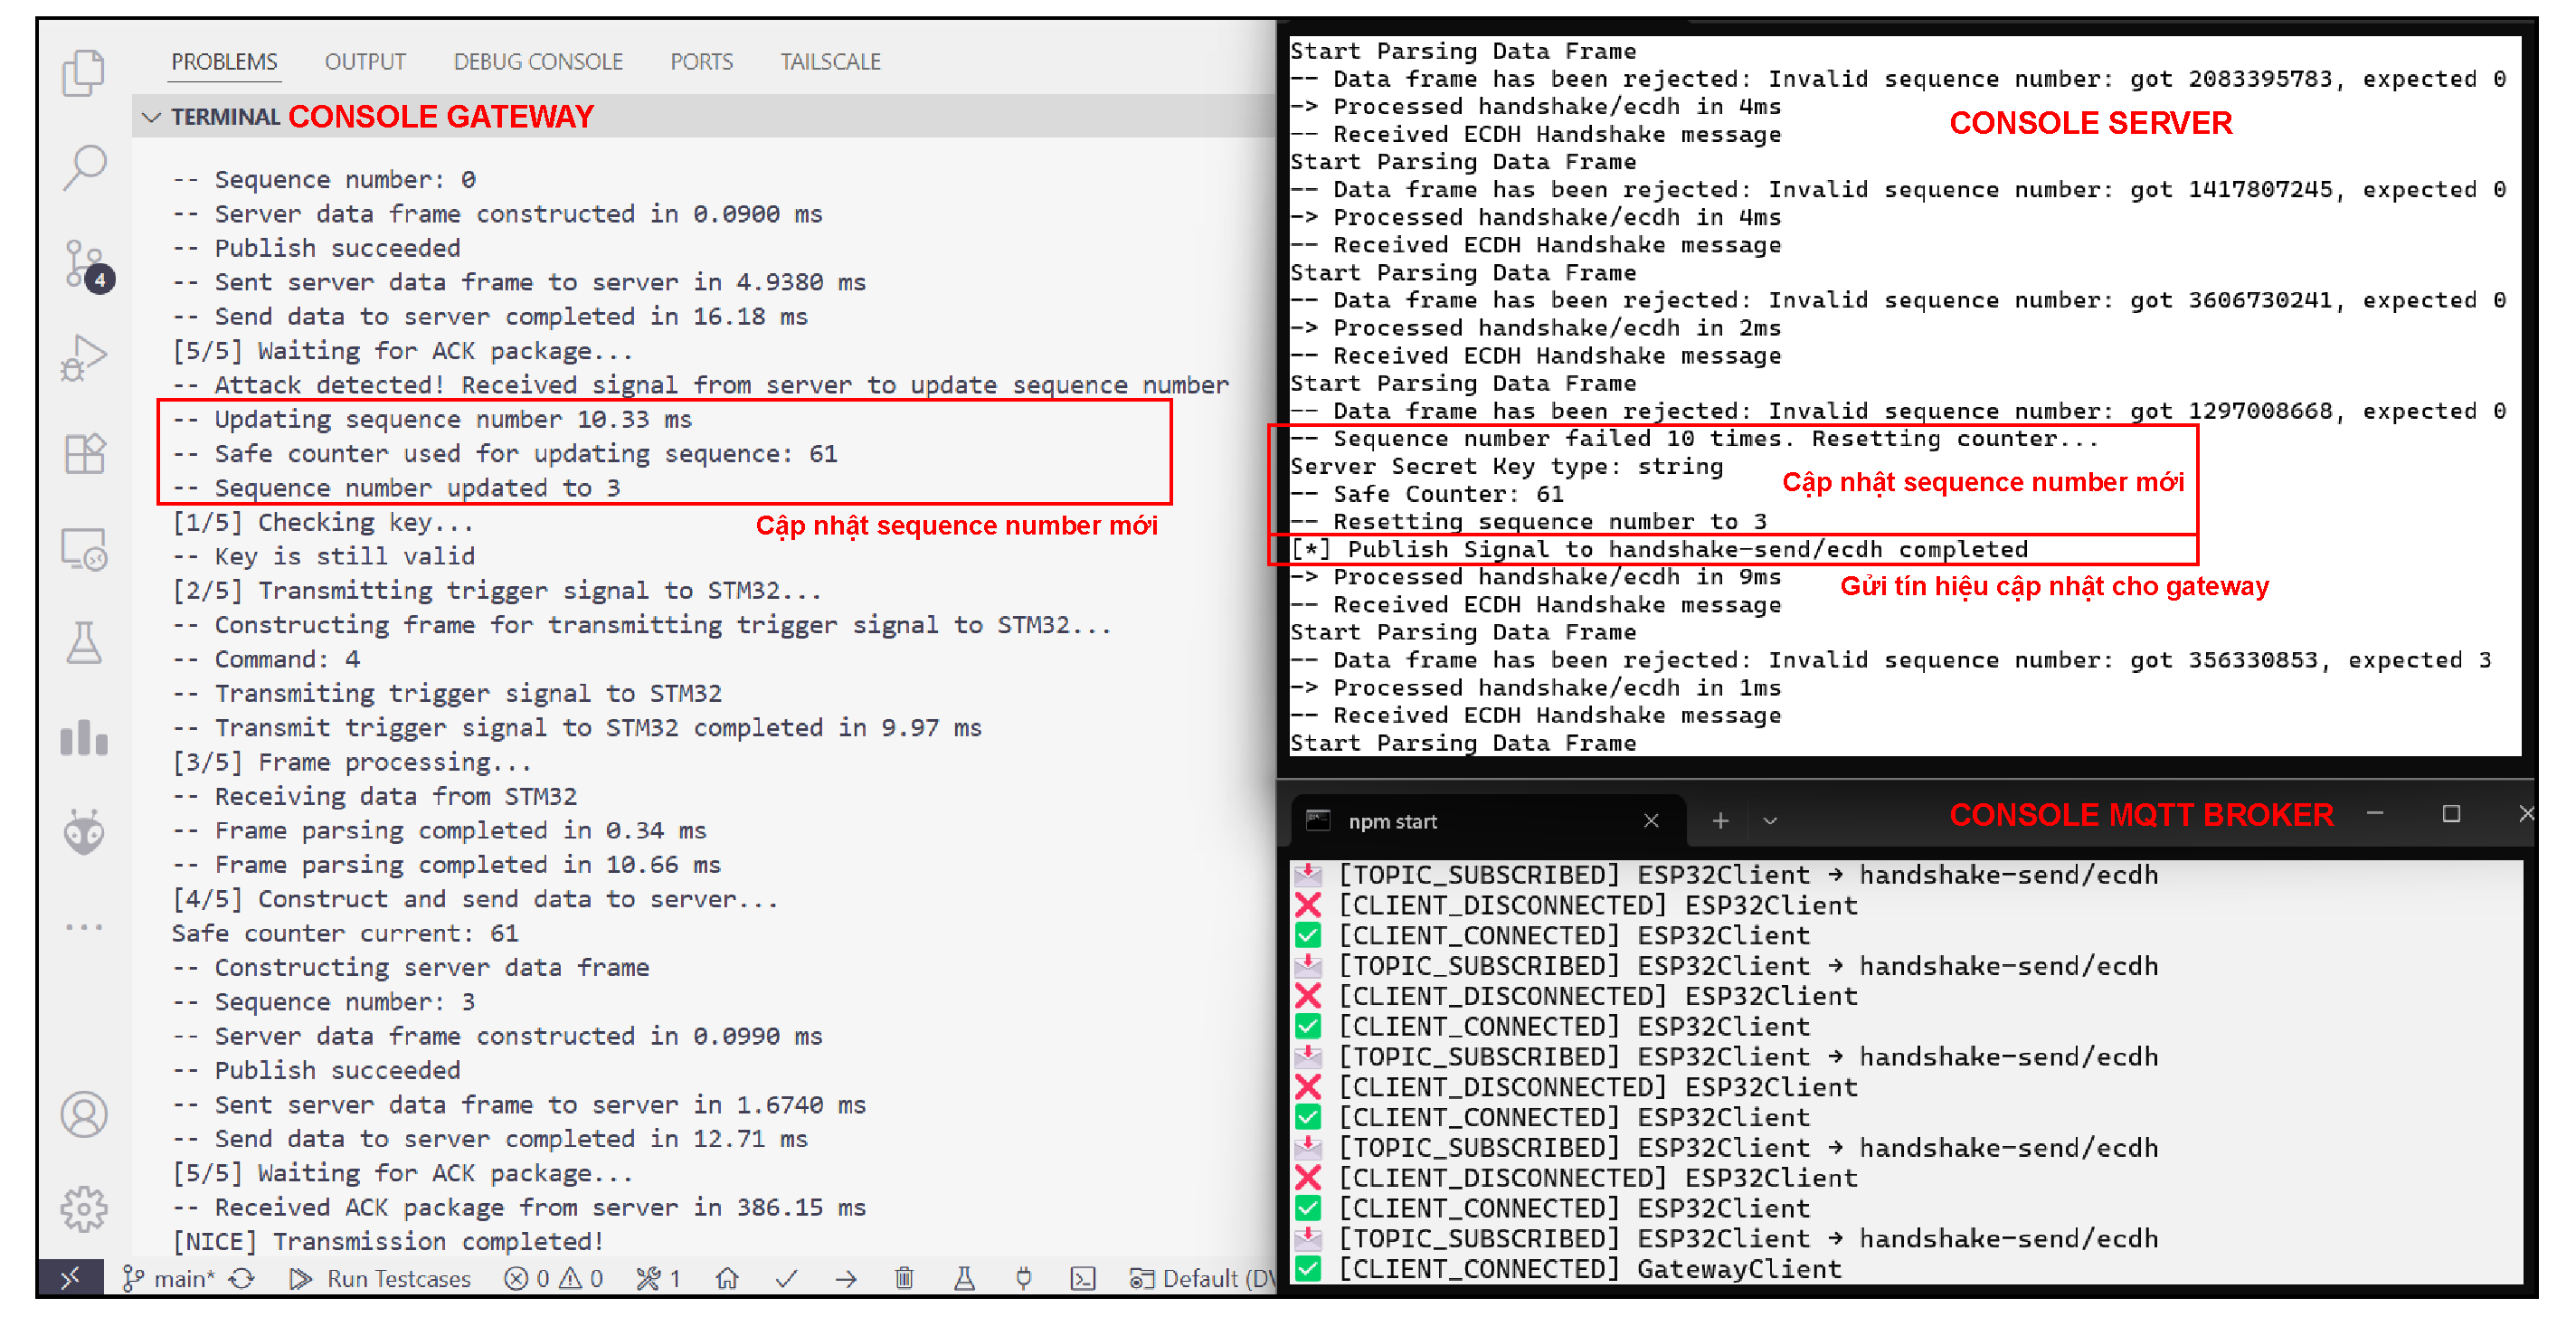
\includegraphics[width=1\linewidth]{sclog.pdf}
%     \caption{Log của gateway và máy chủ trong quá trình cập nhập}
%     \label{fig:sclog}
% \end{figure}

% \subsection{Triển khai máy chủ}
% Máy chủ đóng vai trò trung tâm trong hệ thống IoT, chịu trách nhiệm tiếp nhận dữ liệu từ gateway, xử lý và phân giải các gói tin, kiểm tra tính hợp lệ của gói tin, sau đó cung cấp thông tin đến người dùng cuối. Đối với các gói tin không hợp lệ, máy chủ có khả năng từ chối ngay lập tức để không ảnh hưởng đến người dùng. Trong kiến trúc hệ thống này, máy chủ được cấu hình để thực hiện một số chức năng quan trọng liên quan đến bảo mật và xử lý dữ liệu. Thuật toán trao đổi khóa ECDH được sử dụng để thiết lập khóa chung giữa gateway, trong khi thuật toán Ascon-128a đảm nhiệm việc giải mã và xác thực dữ liệu nhận được. Ngoài ra, máy chủ còn sử dụng hàm băm Ascon Hash nhằm tạo ra khóa phiên cho quá trình giải mã. Hệ thống máy chủ được triển khai trên nền tảng Node.js, với JavaScript là ngôn ngữ lập trình chính, giúp đảm bảo khả năng mở rộng, xử lý bất đồng bộ hiệu quả và dễ dàng tích hợp với các thành phần khác trong hệ thống. Hình \ref{fig:sg} trình bày mô hình giao tiếp giữa gateway và máy chủ sử dụng giao thức MQTT.

% \begin{figure}[H]
%     \centering
%     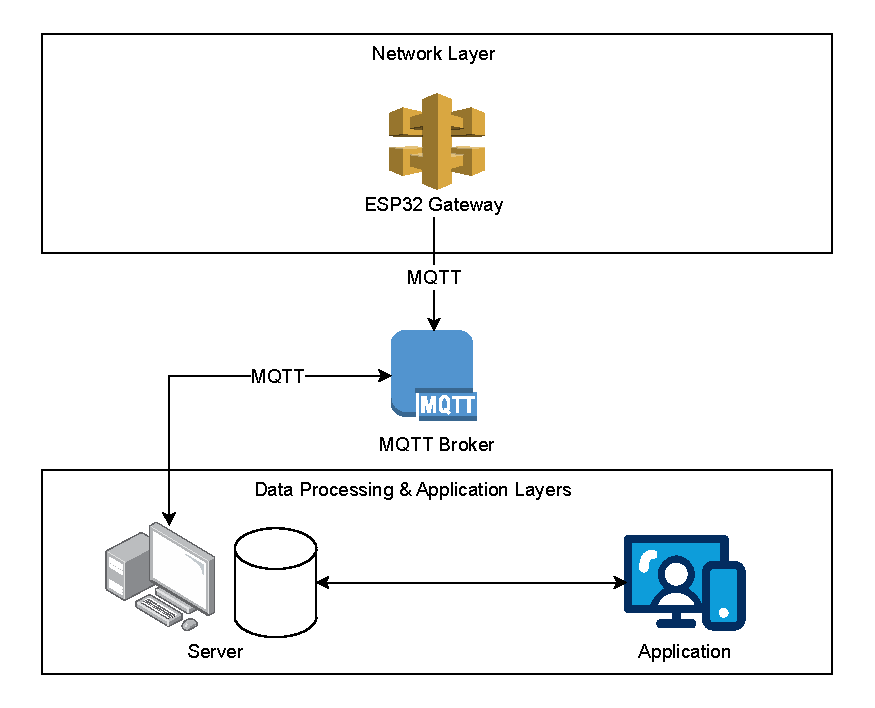
\includegraphics[width=0.75\linewidth]{servergateway.pdf}
%     \caption{MQTT trong giao tiếp giữa gateway và máy chủ}
%     \label{fig:sg}
% \end{figure}